\scanpage{77}
% @0 upper right
\mspage{- 20 -}
% @1–4 continuation
cribles $R\handwritten{\hookrightarrow}X$ couvrant $X$. La deuxième suite spectrale s'en déduit immédiatement et peut d'ailleurs s'interpréter comme une suite spectrale de foncteurs composés (formule (17)). Les assertions sur les morphismes $\handwritten{\Phi}^q$ et $\handwritten{\Phi}^q_X$ s'obtiennent en remarquant que les termes
% @5 display
\[
 \handwritten{\check{\mathscr H}}^0(\handwritten{\mathscr H}^q(F))\qquad q\ne0
\]
% @6 nullity
sont nuls ((2.2) et (formule (23)).

% @7–11 bracketed corollary
\noindent\begin{tikzpicture}
\node[inner sep=3pt] (cor) {\begin{minipage}{.89\linewidth}
\uline{Corollaire 2.6} : (au corollaire 2.5) : Soient $E$ un topos, $A$ un \handwritten{A}nneau de $E$ (commutatif à élément unité), $S$ un objet de $E$, $F$ un $A$-Module. Désignons par $\underline F$ le groupe abélien sous-jacent à $F$. Le foncteur $F\handwritten{\leadsto}\underline F$ est exact et par suite l'isomorphisme canonique :
% @12 degree zero
\[
 H^0(E/S,F)\mathrel{\overset{\handwritten{\sim}}{\relbar\joinrel\handwritten{\rightarrow}}}H^0(E.S,\underline F)
\]
% @13 introduction
définit des morphismes :
% @14 degree q
\[
 H^q(E/S,F)\mathrel{\relbar\joinrel\handwritten{\rightarrow}}H^q(E/S,\underline F)
\]
% @15 conclusion
Ces morphismes sont des isomorphismes.
\end{minipage}};
\handwritten{\draw (cor.north west) ++(2pt,1pt) -- (cor.north west) -- (cor.south west) -- ++(2pt,-1pt);}
\end{tikzpicture}

% @16–19 proof
\uline{Preuve} : On se ramène immédiatement au cas où $E$ est une catégorie de faisceaux sur un site $C\handwritten{\in \underline U}$ dont $S$ est un objet (2.4.14.II). On peut aussi (3.\handwritten{5}.4.III) supposer que les produits fibrés sont représentables dans $C$.
% @20 encircled typed phrase
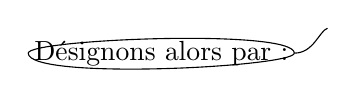
\begin{tikzpicture}[baseline=(phrase.base)]
\node[inner sep=2pt] (phrase) {Désignons alors par :};
\handwritten{\draw[thin] (phrase.east) .. controls +(7pt,0pt) and +(-3pt,-1pt) .. ++(12pt,9pt);
\draw[thin] (phrase.east) .. controls +(0,9pt) and +(0,5pt) .. (phrase.west) .. controls +(0,-10pt) and +(0,-5pt) .. (phrase.east);}
\end{tikzpicture}
% @21 final display
\[
 \handwritten{\mathscr H}^0:\ C_A^{\handwritten{\sim}}\mathrel{\relbar\joinrel\handwritten{\rightarrow}} C_A^{\wedge}
\]
% @22 foot
\hfill \ldots/\ldots
% archive sheet number: 76

